% id: 130-62
% book: 베이직쎈 대수 · 07 삼각함수의 그래프
% section: 개념 48 삼각부등식
% passage: 다음 부등식을 푸시오.
% figure: none
% answer: 
% answer_source: 
% variant_level: 0 (원본 전사)
% 이 파일은 build.mjs 가 items.json 에서 만든다. 고칠 때는 items.json 을 고친다.
\smash{\raisebox{4.5mm}{\dmkichul{베이직쎈 대수 130쪽 62번}}}
$\cos\left(x-\dfrac{\pi}{3}\right)\le-\dfrac{1}{2}$ \dmcondfill{$0\le x<2\pi$}{}
\dmhint{$x-\dfrac{\pi}{3}=\theta$로 놓으면 \quad $\blank\le\theta<\blank$\\ 주어진 부등식은 \quad $\cos\theta\le-\dfrac{1}{2}$\par\smallskip\dispeq{% 130-62(130쪽) — 🎯 힌트 안 그래프: $\theta=x-\frac{\pi}{3}$ 로 놓았을 때 $y=\cos\theta$ $\left(-\frac{\pi}{3}\le\theta<\frac{5}{3}\pi\right)$ 와 직선 $y=-\frac{1}{2}$.
% 스캔 화질이 낮아 TikZ 로 다시 그림. 라벨은 원문에 있는 것만 — $1$·$-1$, $-\frac{\pi}{3}$·$\pi$·$\frac{5}{3}\pi$.
% 원문처럼 직선보다 아래쪽 곡선 부분만 색을 넣었고 그 양 끝 값(답으로 이어지는 값)은 적지 않는다. 왼쪽 끝 닫힌 점·오른쪽 끝 열린 점.
\begin{tikzpicture}[line width=0.6pt, x=0.80cm, y=0.72cm]
  \draw[dotted, line width=0.5pt] (0,-1) -- (3.1416,-1) (3.1416,-0.5) -- (3.1416,-1);
  \draw[->, >=stealth, line width=0.7pt] (-1.65,0) -- (6.45,0) node[above=1pt, font=\footnotesize] {$\theta$};
  \draw[->, >=stealth, line width=0.7pt] (0,-1.70) -- (0,1.80) node[left=1pt, font=\footnotesize] {$y$};
  \draw[line width=0.6pt] (-1.65,-0.5) -- (5.95,-0.5);
  \draw[line width=0.7pt, domain=-1.0472:5.2360, samples=140, smooth] plot (\x, {cos(57.2958*\x)});
  \draw[red!75, line width=0.9pt, domain=2.0944:4.1888, samples=60, smooth] plot (\x, {cos(57.2958*\x)});
  \fill (-1.0472,0.5) circle (1.7pt);
  \draw[fill=white, line width=0.5pt] (5.2360,0.5) circle (1.7pt);
  \fill[red!75] (2.0944,-0.5) circle (1.7pt);
  \fill[red!75] (4.1888,-0.5) circle (1.7pt);
  \node[anchor=east, font=\footnotesize] at (-0.12,1) {$1$};
  \node[anchor=east, font=\footnotesize] at (-0.12,-1) {$-1$};
  \node[anchor=east, font=\footnotesize] at (-1.40,0.52) {$-\dfrac{\pi}{3}$};
  \draw[->, >=stealth, line width=0.4pt] (-1.36,0.46) -- (-1.12,0.46);
  \node[anchor=north east, font=\footnotesize] at (-0.06,-0.06) {$\pt{O}$};
  \node[anchor=south, font=\footnotesize, fill=white, inner sep=0.6pt] at (3.1416,0.05) {$\pi$};
  \node[anchor=south, font=\footnotesize] at (5.42,0.62) {$\dfrac{5}{3}\pi$};
  \draw[->, >=stealth, line width=0.4pt] (5.42,0.58) -- (5.28,0.42);
  \node[anchor=north, font=\footnotesize] at (2.70,-1.06) {$y=\cos\theta$};
  \node[anchor=west, font=\footnotesize] at (6.00,-0.5) {$y=-\dfrac{1}{2}$};
\end{tikzpicture}
}\par\smallskip\noindent $\cos\theta\le-\dfrac{1}{2}$의 해를 구하면 \quad $\blank\le\theta\le\blank$\\ 즉 $\blank\le x-\dfrac{\pi}{3}\le\blank$이므로 \quad $\blank\le x\le\blank$}
